\chapter{Fundamentação Teórica}
\addcontentsline{toc}{chapter}{Fundamentação Teórica}

\section{Aprendizado de Máquina}
Aprendizado de máquina é uma disciplina focada em duas questões interelacionadas: Como construir sistemas que automaticamente melhoram por meio da experiência? e quais as leis estatisticas,
computacionais e da teoria da informação que governam todos os sistemas de aprendizagem, incluindo computadores, seres humanos, e organizações?. O estudo de aprendizado de máquina é importante tanto
para responder a essas questões fundamentais de Engenharia e Ciência, quanto pelas aplicações computacionais que tem produzido \cite{Jordan}.
Um problema de aprendizado, pode ser colocado como um problema que reside em melhorar uma medida de performance, quando se executa alguma tarefa, através de algum tipo de experiência de treinamento \cite{Jordan}.

Uma tarefa pode ser entendida como o processo de categorizar um dado, que será utilizado como entrada do algorítmo de aprendizado de máquina escolhido. Um bom exemplo dado por \cite{Jordan}, é a classificação de uma
transação bancária como fraudulenta ou não. A tarefa reside exatamente na categorização. O quão precisa essa categorização é, depende da forma como o algorítmo escolhido para atender tal demanda é treinado. A maneira como
esses dados são categorizados varia de acordo com o algorítmo selecionado para a classificação. Cada algorítmo espera que esses dados sejam modelados de uma forma ou de outra, assunto que será abordado ao longo deste capítulo.

\subsection{Aprendizado Estatístico}
Podemos definir então, que a entrada do nosso algorítmo será um conjunto de dados representados aqui pelo simbolo X, e a nossa saída sendo representada pelo simbolo Y. 
X pode ser chamada de diversas formas, como preditor, variáveis independentes, características ou simplesmente variáveis. 
O simbolo Y é normalmente chamado de resposta, ou variável dependente. Se consideramos um segundo exemplo dado por \cite{James}, em que o salário de um indivíduo é deduzido a partir
de fatores como a sua idade, escolaridade e o ano em que os dados foram coletados. Temos que $X = \{idade, escolaridade, ano\}$, enquanto Y representa o salário, ou seja, o fator que varia,
conforme $X_1(idade)$  ,$X_2(escolaridade)$ e $X_3(ano)$ variam. Poderiamos ter $p$ variáveis para $X$, nesse caso $p$ é igual a 3.
Podemos então representar essa relação entre $X$ e $Y$ da seguinte forma:

\[
  Y = f(X) + e
\]

Nessa formulação $f$ é uma função fixa mas desconhecida de $X_1...X_p$, e $e$ é o termo de erro randomico, que é independente de $X$ e tem media zero. Essa formulação pode ser dita
como ideal e teórica, uma vez que a função $f$ utilizada na prática, e o valor $Y$ encontrado como resultado, são estimativas, construidas a partir do aprendizado estatístico.
Nessa formulação, $f$ representa a informação \textit{sistematica} que $X$ provê em releação a $Y$\cite{Jordan}.  
Para definirmos $f$ devemos primeiro compreender a diferença entre inferência e predição.
\subsubsection{Predição}
Quando o objetivo do aprendizado reside em deduzir ou estimar um valor de $Y$, dado $X$, temos uma situação de predição. Podemos realizar essa predição utilizando 
\[
  Y^* = f^*(X)
\]

$f^*$ é a estimativa para $f$, $Y^*$ é o valor previsto para $Y$. A precisão de $Y^*$ como uma previsão de $Y$ depende de dois valores, chamados de \textit{erro reduzivel} e \textit{erro irreduzivel}. No geral, $f^*$ não será uma estimativa perfeita de $f$, e essa imperfeição irá naturalmente, adicionar erros no resultado\cite{Jordan}.
\subsubsection{Inferência}


A disciplina de aprendizado de máquina pode ser subdividida da seguinte forma:
\begin{figure}[h]
	\centering
	\label{fig01}
        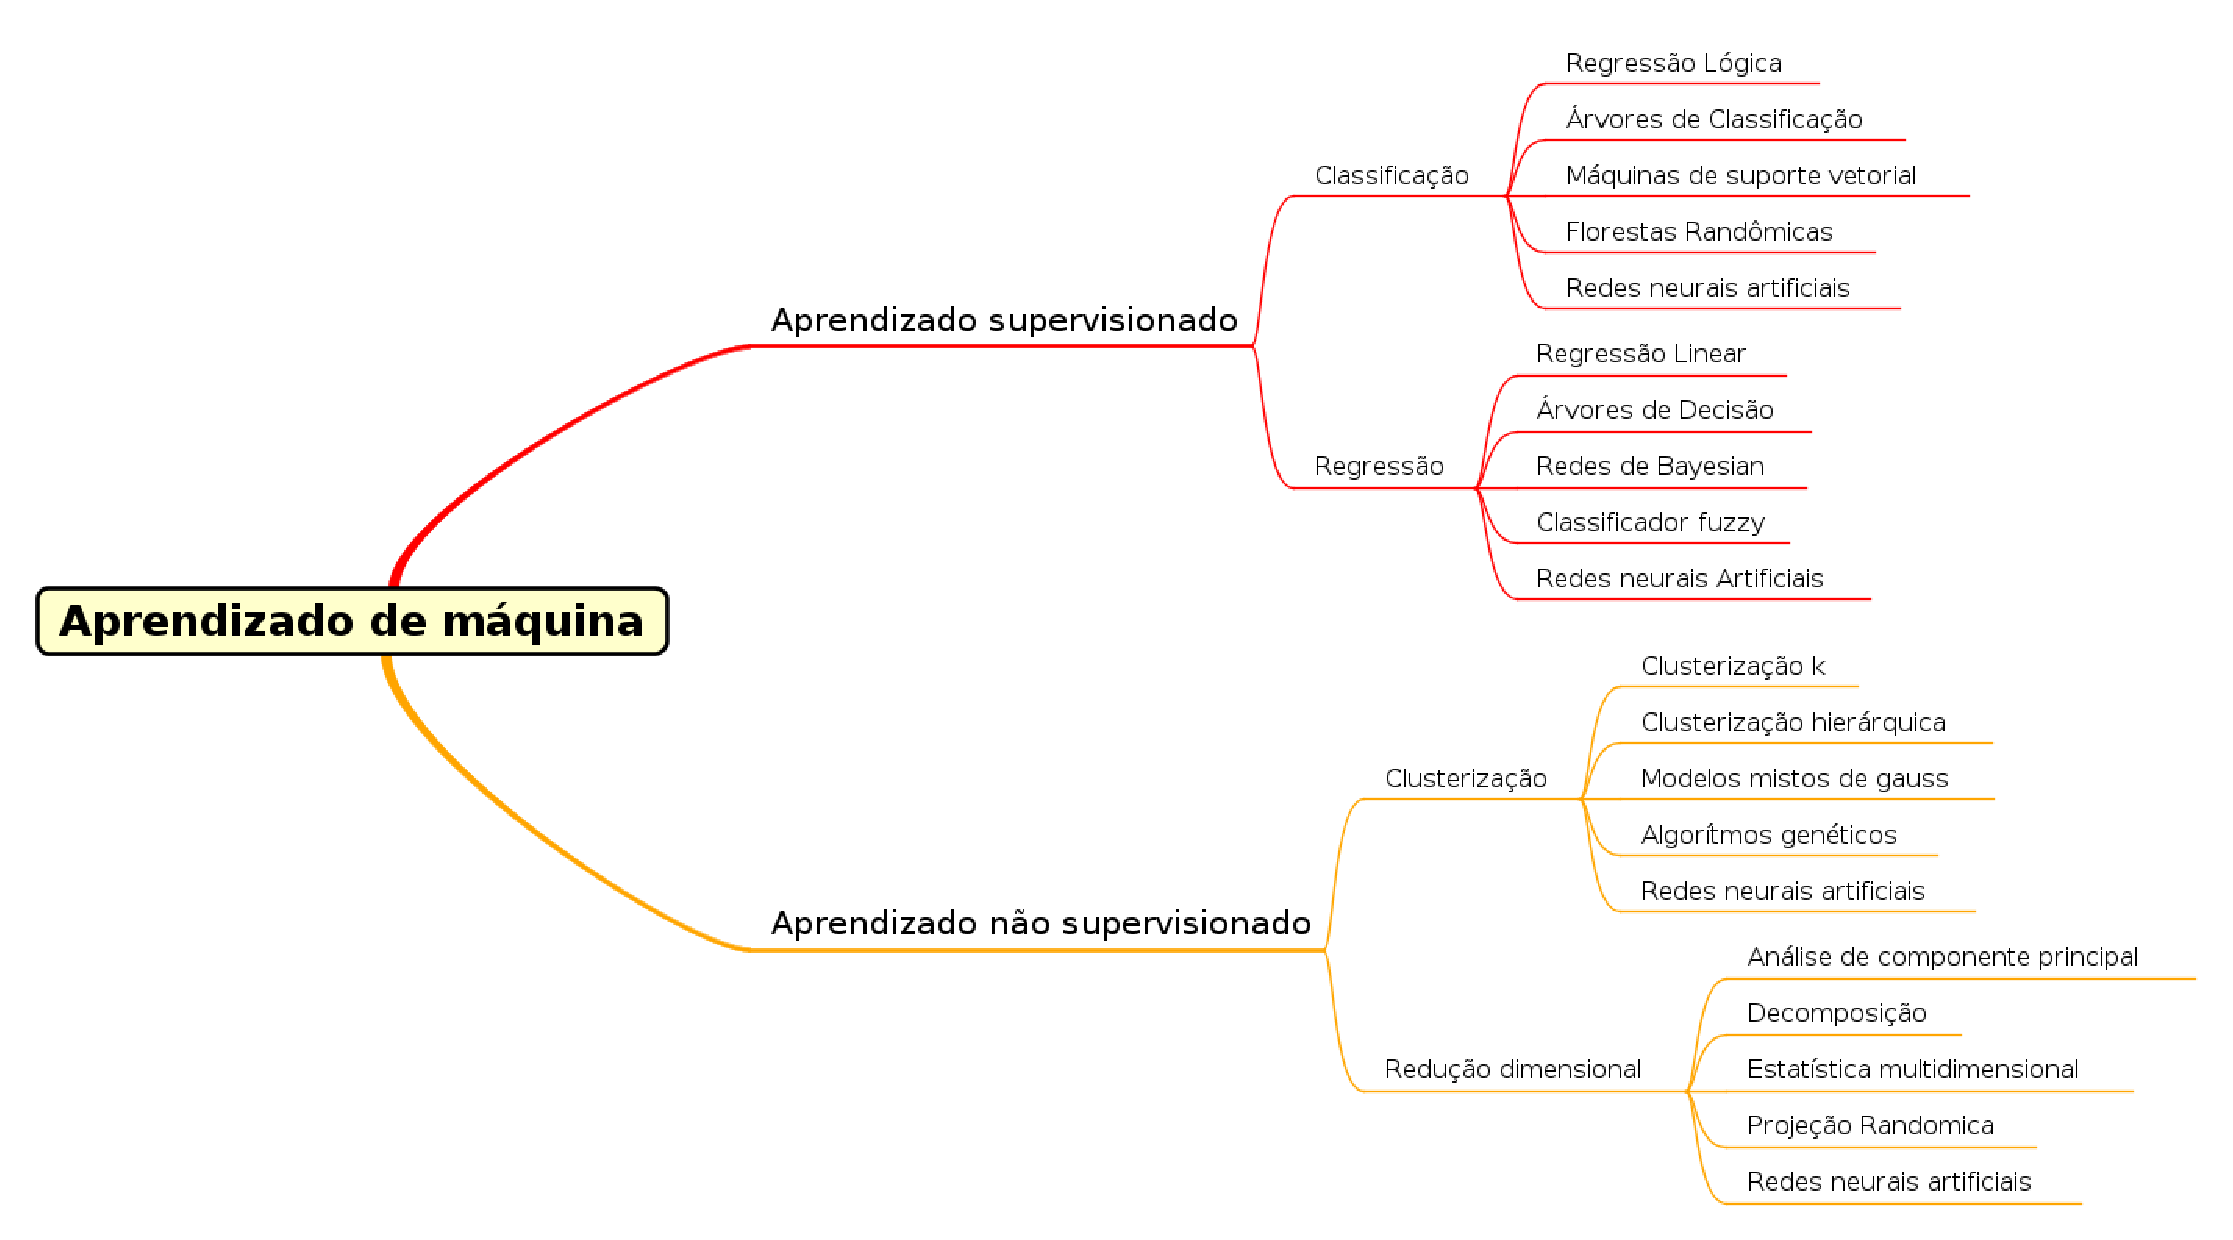
\includegraphics[scale=0.33]{figuras/mind1.eps}
	\caption{Abordagens para aprendizado de máquina}
\end{figure}
Neste capitulo iremos direcionar nossos estudos para o aprendizado supervisionado, pois eles são a base para sistemas de classificação.

\subsection{Aprendizado supervisionado}
Para o aprendizado supervionado, o conjunto de dados utilizado no treinamento será formado pelos dados em si, e pela saída esperada para esses dados\cite{Louridas}. Segundo \cite{James}, aprendizado estatístico supervisionado involve construir um modelo estatístico para prever ou estimar, uma saída a partir de uma ou mais entradas.  É no ambito do aprendizado supervisionado,
que sistemas de classificação são construidos. Para que um sistema de classificação, classifique dados desconhecidos, é preciso treina-lo com um conjunto de dados em que cada dado, possui sua classificação previamente definida.  O conceito de melhorar a experiência no aprendizado de máquina, reside justamente no aprendizado supervisionado.

\subsubsection{classificação}

\subsubsection{regressão}

\subsection{Modelo estatístico}

\subsection{Sistemas de classificação}
Sistemas de classificação são largamente utilizados na indústria e na academia. Estudos em diferentes áreas do conhecimento
lançam mão de algorítmos de aprendizado de máquina para extrair valor de dados que não necessáriamente são totalmente objetivos. Na realidade,
técnicas de aprendizado de máquina, são tolerantes a dados que são imprecisos, parcialmente incorretos ou incertos \cite{Malhotra}. .


% TODO: Trazer mais um exemplo de sistemas de classificação

Para construir um sistema de classificação é imprecindivel a definição de um modelo estatístico que represente o sistema complexo em que estamos inseridos, e a utilização de um classificador, que ao ser treinado a partir do modelo, pode vir a classificar dados novos. Dizemos que o modelo representa um sistema complexo, justamente lidar com diversas variáveis distintas, e que podem, estatisticamente falando, terem influência uma sobre as outras.
